% Template for ICIP-2017 paper; to be used with:
%          spconf.sty  - ICASSP/ICIP LaTeX style file, and
%          IEEEbib.bst - IEEE bibliography style file.
% --------------------------------------------------------------------------
\documentclass{article}
\usepackage{spconf,amsmath,graphicx}
\usepackage{subcaption}

\usepackage{pgfplotstable}
\usepackage{pgfplots}

\captionsetup[figure]{font=small,skip=0pt}


% Example definitions.
% --------------------
\def\x{{\mathbf x}}
\def\L{{\cal L}}

% Title.
% ------\title{Ambiguity Index for Stereo Reconstruction Based on Dynamic Programming}
\title{Ambiguity Index for Semi-Global Matching based Stereo Reconstruction }
%
% Single address.
% ---------------
\name{Mathias Paget, Jean-Philippe Tarel\thanks{Thanks to FUI AWARE project for funding.}}
\address{
Universit\' e Paris-Est, \\
 COSYS, LEPSIS, IFSTTAR, \\
F-77447 Marne-la-Vall\' ee, France}


\begin{document}
\ninept
%
\maketitle
%

\begin{abstract}
Stereoscopic reconstruction is an important task for automatic vision systems. This task being a step, estimating the reconstruction is not enough and its uncertainty must be characterized for correct performance of the whole system. Several methods proposed uncertainty indexes based on well chosen data features, thus incomplete. Other methods were proposed based on leaning. We here propose a simple index, we named ambiguity index, which takes into account data and regularization as well, and which is derived only from the data generated during the optimization process, by exploiting interesting properties of the dynamic programming (DP). This index is an approximate of the posterior variance when Semi-Global Matching (SGM) algorithm is used for stereo reconstruction. To evaluate the proposed index, we show improvements when it is used to refine the stereo reconstruction on the KITTI databases~\cite{geiger13, menze15}.
\end{abstract}
\begin{keywords}
Stereo reconstruction, Discrete optimization, Dynamic Programming, Semi-Global Matching, Uncertainty index
\end{keywords}

\section{Introduction}
\label{sec:intro}

An accurate and robust perception of the environment is required for Advanced Driver Assistance Systems (ADAS) and Automatic driving to perform and schedule driving tasks. When only cameras are used for perception, many driving tasks, where the system needs to build high-level information form low-level image information, are known to challenge computer vision and image processing. To face these difficult and complex problems, tasks are usually decomposed into a chain or a tree of sub-problems, each sub-problem being handled by an image or computer vision process. In such kind of approach, the output of each process is the input of another one. Usually, each process is set as the minimization of an energy. The advantage of the decomposition into sub-problems is that the propagated information is reduced along the chain or the tree, however the risk is to reduce too drastically the propagated information and to lead to inconsistent results. To solve this issue it is necessary to propagate uncertainty information in addition to the estimation result to allow the next process to integrate it along the processing chain or tree. In this article, we focus on stereoscopic reconstruction of road scenes.

When the input noise is Gaussian and the problem is linear and well-posed, the uncertainty of the output is shown to be a Gaussian function characterized by the co-variance matrix of the output. This covariance matrix can be formally derived from the minimized energy. When the input noise is not Gaussian, or when the problem is non-linear, the uncertainty of the output can be approximated by a Gaussian function, but derived co-variance matrix may be voluminous. Thus, only problems with a reduced number of parameters, such as for instance camera calibration, can be handled but not stereo-reconstruction where the number of parameters is usually over one million. Rather to estimate the co-variance matrix of the output, it was thus proposed for stereo-reconstruction to estimate an uncertainty index based on the data features which are known to harden resolution of the problem, such as texture-less regions, repetitive patterns~\cite{hu12}. The difficulty of this approach is that it is hard to fully understand data's effect on the estimated solution due to the usual regularization term used during stereo-reconstruction minimization.
This why it was proposed in~\cite{haeusler13, spyropoulos14, park15, seki16} to learn confidence on the solution form feature on data, data cost and disparity map estimate.

Instead of trying to learn it, we investigate the possibility to build an index only from the energy and from what is computed during the optimization process. It appears that optimization methods based on dynamic programming such as the discrete optimization method called Semi-Global Matching (SGM) first introduced in~\cite{hirschmuller08}, have very interesting properties which allows us to estimate easily an index on the solution, we named ambiguity index. As the ambiguity index comes from intermediate costs computed during the optimization, it needs a very reduced amount of computations to be obtained. The proposed ambiguity index is evaluated by several experiments to show its interest. It is in particular used to refine the stereo-reconstruction estimate to show its ability to improve results and thus to reduce reconstruction errors.

\section{Stereo Reconstruction}
\label{sec:index}

The used stereo reconstruction algorithm is a simplified version of~\cite{zbontar16} where input images are assumed with rectified geometry. Following~\cite{scharstein02}, we describe the stereo reconstruction algorithm split into four steps: matching cost computation in Sec.~\ref{ss:cost}, cost aggregation in Sec.~\ref{ss:cost}, optimization in Sec.~\ref{ss:sgm} and refinement in Sec.~\ref{ss:lr_cons}.

\subsection{Matching Cost and Aggregation}

\label{ss:cost}

In the rectified geometry, object depth is easily parameterized by the difference in horizontal position between its left and right projections, the so-called disparity. Stereo-reconstruction problem is usually set as the minimization, with respect to the disparity image, of an energy which is a function of the left and right images. The Bayesian approach provides ways to derive this energy from a statistical model of the stereo reconstruction problem. Let's considering an energy of the form:
\begin{equation}
E(D) = \sum_{p \in P}{Data(p,d_p)} + \sum_{(p,q) \in N}{Prior(d_p,d_q)}
\label{eq:global_en}
\end{equation}
where $D=(d_p)$ is the disparity image, $d_p$ the disparity of the pixel $p$, $P$ is the pixel set, $N$ the set of neighboring pairs of pixels. Data term $Data$ describes how data agrees with the solution and a prior term $Prior$ describes the wanted properties of the solution. In our case, $Data$ is set to the census dissimilarity~\cite{zabih94} between left and right pixel patches, assuming that the two projections look alike in a neighborhood. The census is computed on a 5*5 window and its advantage is invariance to an increasing function on the intensities, so it can handle photometric calibration differences between the two images and partially perturbations due to aspect differences depending of the viewing angle. Like in~\cite{zhang09}, cross-based aggregation is performed on the data cost. By smoothing the data cost in regions of homogeneous intensities, the noise is reduced in the data cost and thus also in the solution.

The term $Prior$ is set to a function of the disparity difference, assuming that two neighbor pixels have same depth (also called front-parallel prior). The assumption on the data term is non completely valid due to occlusion, reflexions and specularities as well as for the prior term due to no-frontal surfaces such as road and lateral buildings. Intents to perform more accurate modeling, for instance to handle occlusion~\cite{kolmogorov01} or regularization with higher order prior~\cite{ranftl12}, lead to more difficult to optimize energies. For this reason, simple energies are often preferred and erroneous pixels of the solution are post-processed. In practice, $Prior$ function is set to:
\begin{equation}
\begin{split}
Prior(i,j) = 0, & \; \; if \; i=j, \\
Prior(i,j) = P1, & \; \; if \; |i-j| = 1, \\
Prior(i,j) = P2, & \; \; otherwise.
\end{split}
\end{equation}
It thus behaves close to a $Pott$ regularization function, yet is more permissive for slow disparity variations. This allows to better handle road scene where non-frontal plan are numerous such as the road and lateral buildings.

\subsection{Semi-Global Matching Optimization}
\label{ss:sgm}

The energy defined in (\ref{eq:global_en}) is a 2D first order Markov Random Field (MRF). Global optimization of a such energy is difficult, so approximated optimization algorithms have been proposed. With Semi-Global Matching (SGM), introduced in~\cite{hirschmuller08}, the original energy is decomposed in many 1D energies where a global optimum can be found. SGM thus consists in minimizing along "arms" around each considered pixel using Dynamic Programming (DP). For each pixel, vector direction $v$, a 1D energy $C_v$ is computed using the following recursion rule:
\begin{equation}
\begin{split}
C_v(p,d) = & Data(p,d) + \\
& \min_{d'}{ C_v(p-v,d') + Prior(d,d')}.
\end{split}
\end{equation}
The original $SGM$ is performed along 16 directions. We consider only 4 directions as in~\cite{zbontar16}, fostering horizontal and vertical directions in the optimization achieves better results for vertical and horizontal scene objects. The four energies $C_v$ are added at the current pixel and the estimate is selected at the minimal value of this energy over disparities:
\begin{equation}
\begin{split}
SGM(p,d) & = \sum_{v} C_v(p,d) - (R-1)Data(p,d) \\
Solution(p) & = arg\min_{d}{SGM(p,d)}
\end{split}
\end{equation}
where $R=4$ is the number of considered directions. Because of the 1D decomposition, each pixel solution is obtained independently and thus the smoothness of the solution is not guaranteed, despite the regularization term. This leads to SGM artifacts. By smoothing the data cost, cross based aggregation reduces these artifacts.

\subsection{Left-Right Consistency (LRC) refinement}
\label{ss:lr_cons}

Since the model is not always valid in particular at occlusions, an additional prior is introduced during post-processing, the so-called Left-Right Consistency (LRC) on disparities~\cite{mei11}. The idea is to check that for the same object point, the disparity in the left and right images are the same. LRC check consists in comparing the disparity, of a given pixel, to the disparity at corresponding position in the other image. Three pixel categories are thus defined:
\begin{equation}
\begin{split}
correct, & \; |d - D_r(p- d)| \leq 1, \; for \; d=D_l(p) \\
mismatch, & \; |d - D_r(p- d)| \leq 1, \; for \; any \; other \; d \\
occlusion, & \; otherwise.
\end{split}
\end{equation}
A processing on the result is performed depending of the LRC category like in~\cite{zbontar16}. For "Correct" pixels, the solution value is not modified. For "Occlusion" pixels, its value is set to the value of the first "correct" pixel at its left, thus occluded pixels are set to the background. For "Mismatch" pixels, the value is set to the median value of the nearest "correct" neighbors in 8 directions (originally 16).

\section{Ambiguity Index}

Learning approaches were proposed recently to estimate the confidence of the solution in the context of the stereo reconstruction. Confidence has to be understood as a prediction of an error on matching over a given threshold. It is learned from data, data cost and estimated disparity map features~\cite{spyropoulos14, park15, seki16} and additionally from final SGM cost~\cite{haeusler13}. Theses four approaches require learning and a large ground-truth database, so we aim to propose an uncertainty index only using sub-products of the optimization process itself, we named ambiguity index.

\subsection{Posterior Variance for SGM}

The a priori variance is evaluated from the data cost only, yet it does not provide useful information on the solution. This is why well selected features from input data were proposed to partially characterize the data uncertainty~\cite{hu12}. As the estimated solution is an agreement between data and prior costs, it is quite hard to derive all the good features. The posterior variance of the estimated solution is the right characterization, since it takes into account data and prior costs. However, its estimation for a 2D RMF such as energy (\ref{eq:global_en}) is a very complex task. Indeed, the posterior covariance is a quadratic approximation of the shape of the energy (\ref{eq:global_en}) around the obtained solution which is assumed at a local minimum of this energy. Due to the large number of parameters, the computation of this quadratic approximation is intractable.

Instead of evaluating the posterior variance of the original energy, since we are using SGM optimization, we better work on the SGM cost. As recalled previously, the SGM optimization decomposes and approximates the 2D problem into many 1D problems. Additionally, we exploit one important property of the DP: each value in the DP final cost, thus after DP optimization, is the minimal energy of the original problem with an extra constraint on the solution. For the SGM, this implies that each value of the $SGM$ final cost is the minimum value of the following sub-problem: considering the set $X_p$ of pixels within the horizontal and vertical "arms" from the pixel $p$, $SGM(p,d)$ final cost is equal to the minimum cost over $X_p$, with the constraint that the disparity value at $p$ equals $d$. More formally:
\begin{equation}
\begin{split}
  SGM(p,d) = \min_{d_x, x \in X_p | d_p = d} \{  \sum_{i \in X_p}  Data(i,d_i) & \\
  +  \sum_{(i,j) \in N, i \in X_p, j \in X_p} Prior(d_i,d_j) \}  &.
\end{split}
\end{equation}
SGM final cost can be seen as an approximation of the energy (\ref{eq:global_en}) where each final pixel disparity becomes independent for the others. This allows to forget about the posterior covariance between different pixels and to focus only on the pixels posterior variance. The pixel posterior variance is estimated using ambiguity index as the size of the final SGM valleys along disparities:
\begin{equation}
Index(p) = \sum_{d}{|SGM(p,d) - \min_{d'}{SGM(p,d')} < T_1|}
\end{equation}
where $T_1$ is a positive given threshold. A index value of one means that there is no ambiguity. From experimentation, the profile of the final $SGM$ cost is usually with a single valley, so the difference between counting value under the threshold and the value of the difference between maximal and minimal argument under the threshold is small. The proposed index looks similar to perturbation
measure prosed in~\cite{merrell07} in the context of plane-sweeping stereo. In practice, $T_1$ is set at a factor of the $P2$ value used in the regularization term. This link between $T_1$ and $P2$ leads to invariance of the index when a scale factor is applied to the energy. Notice also that the estimated result and ambiguity index derive from the same energy, so a change in the energy affects both of them. It has a very reduced extra computational cost.


\subsection{Index integration into the stereo process}
\label{ss:in_proc}

A way to evaluate index relevance is to use it to refine the reconstruction and to test if the solution is improved. We propose two possibilities. The first one is a post-processing similar to LRC filtering~\ref{ss:lr_cons}), where pixel whose index is under a threshold $T_2$ are set to "correct" label. As the index is not able to distinguish "mismatch" and "occlusion", all others pixels are handled as "mismatch" and set to the median value of nearest "correct" neighbors in 8 directions.

The confidence obtained from learning has be used as a weight in the data cost~\cite{park15} or regularization cost~\cite{spyropoulos14} to balance data and regularization terms. In~\cite{seki16}, an extra regularization term is added in function of the confidence value. The second investigated possibility is to reweight the data term using index inverse:
\begin{equation}
New \; Data(p,d) = \frac{K*Data(p,d)}{Index(p)}
\end{equation}
where $K$ is a constant to maintain global balance between data and regularization terms. Then, a second SGM optimization is performed with this new data cost.

\section{Experiments}
\label{sec:experimentation}

We use stereo rectified images pairs of the databases KITTI 2012~\cite{geiger13} and KITTI 2015~\cite{menze15}. Being not learned, the index is only evaluate on training sets with ground-truth. We Use criterion are the ones of KITTI with the difference that "Non-occulted" ground truth points are enforce to be seen into the two images. The same parameters are used for KITTI 2012 and 2015, color images of KITTI 2015 being converted to grey scale before processing. Regularization parameters $P1$, $P2$ are set to $1.2$, $23$.

\subsection{Ambiguity index as an occlusion prediction}

\begin{figure}[h!]
\begin{center}
\begin{tikzpicture}[scale=0.8, every axis/.style={xmax=30,xmin=1}]
\begin{axis}[xlabel=index values]    
	%xlabel style={at={(current axis.right of origin)}, xshift=18ex, anchor=center}]
	%,ylabel=proportion of pixel
\addplot[ybar interval,mark=no, blue] table [y=correct, x=I]{Figures/histo_12n.dat};
\addlegendentry{"correct"}
\addplot[ybar interval,mark=no, orange] table [y=mismatch, x=I]{Figures/histo_12n.dat};
\addlegendentry{"mismatch"}
\addplot[ybar interval,mark=no, red] table [y=occulted, x=I]{Figures/histo_12n.dat};
\addlegendentry{"occulted"}
\end{axis}
\end{tikzpicture}
\end{center}
\caption{Normalized histograms of index values for the three pixel labels ("correct", "mismatch", occulted") after LRC for all the left image of KITTI 2012 training set. The "correct" mod is at $index=7$, whereas "mismatch" mod is at $index=12$ and "occulted" mod at $index=13$.}
\label{fig:histo}
\end{figure}

When the reconstruction model is not valid, we expect data not to agree with this model and thus that the solution shows a high ambiguity index value, especially at occlusion. We thus compare the ambiguity index with the LRC pixel label. Fig.~\ref{fig:histo} shows the result on KITTI 2012 training set. Despites the overlapping between the three histograms, considering ambiguity index as an non "correct" label predictor gives a $77.7\%$ recall for a $50\%$ precision, thus an over detection by a factor two. This is interesting as ambiguity index has not been designed especially to be an occlusion predictor.
% and LRC labels depend on the reconstruction quality. 

We now consider pixels with an index value higher than $T_2=20$ to be a "mismatch" in the first refinement method proposed in Sec.~\ref{ss:in_proc}. Error rates with the ground-truth are shown in Tab.~\ref{tab:KITTI}. Results before and after standard LRC refinement are also shown. The error rates with LRC and Refinement 1 alone are similar and this suggests that the ambiguity index is a good predictor of non "correct" pixels. When the LRC refinement is applied to the output of Refinement 1, results are slightly improves. This implies that if LRC and Refinement 1 have a shared effect, there are also slightly complementary.

\begin{table}
\centering
\begin{tabular}{|l|c|c|}
  \hline
  Error rate (\%) & Before & After \\
  KITTI2012 / KITTI2015      &  LRC refinement & LRC refinement \\
  \hline
  Original (without index) & 6.13 / 5.23 & 5.13 / 4.45 \\
  Refinement 1 & 5.38 / 4.77 & 4.85 / 4.35 \\
  Refinement 2 & 5.23 / 4.55 & 4.58 / 4.04 \\
  \hline
\end{tabular}
\caption{Average percentage of disparities below 3 pixels error from the "non-occulted" ground truth KITTI 2012 and KITTI 2015 training sets. Refinement 1 is LRC pixel refinement whose index is over $20$. Refinement 2 divides the data cost by the ambiguity index before a second SGM optimization.}
\label{tab:KITTI}
\end{table}

\begin{figure}
\begin{center}
\begin{tikzpicture}[scale=0.8]
  \begin{axis}[view={0}{90}, colorbar, colormap/cool, point meta min=0, point meta max=3000000,
  xlabel=left index values, ylabel= right index values]
    \addplot3[surf] file {Figures/mat.dat};
  \end{axis}
\end{tikzpicture}
\end{center}
\caption{For all "correct" matches of the KITTI 2015 training set, co-occurrence of ambiguity index value in the left and the right image are shown. Notice how left and right ambiguity index are close when disparity matches.}
\label{fig:LR_ind}
\end{figure}

Fig.~\ref{fig:LR_ind} shows the values of the left and right ambiguity indexes for pixels labeled "correct" by LRC. Notice how there is a good correspondence between the left and the right ambiguity index. Therefore, when disparities are consistent, ambiguity index is also consistent between left and right images.

%\begin{figure}
%\centering
%        \begin{subfigure}[t]{0.98\linewidth}
%                \includegraphics[width=0.99\linewidth]{Figures/03}
%                \caption{}
%        \end{subfigure}
%        \begin{subfigure}[t]{0.98\linewidth}
%                \includegraphics[width=0.99\linewidth]{Figures/Occ_03}
%                \caption{}
%        \end{subfigure}        
%        \begin{subfigure}[t]{0.98\linewidth}
%                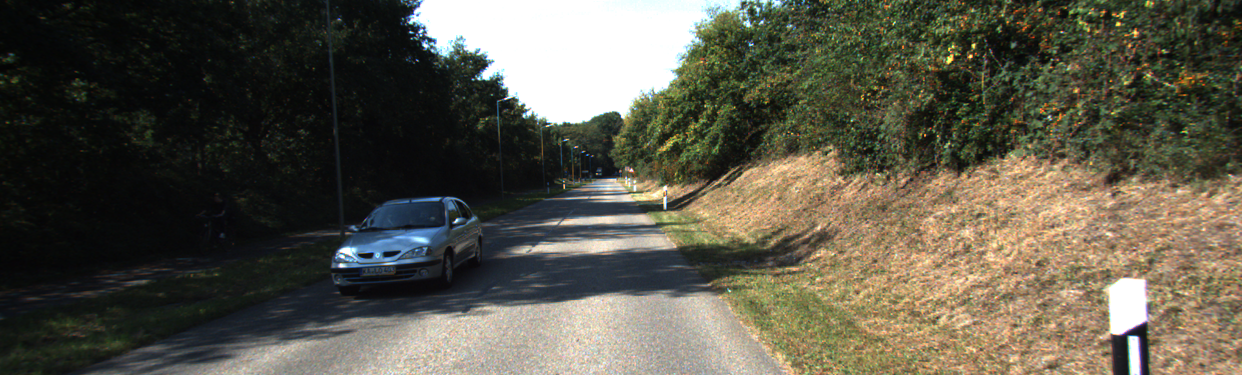
\includegraphics[width=0.99\linewidth]{Figures/56}
%                \caption{}
%        \end{subfigure}
%        \begin{subfigure}[t]{0.98\linewidth}
%                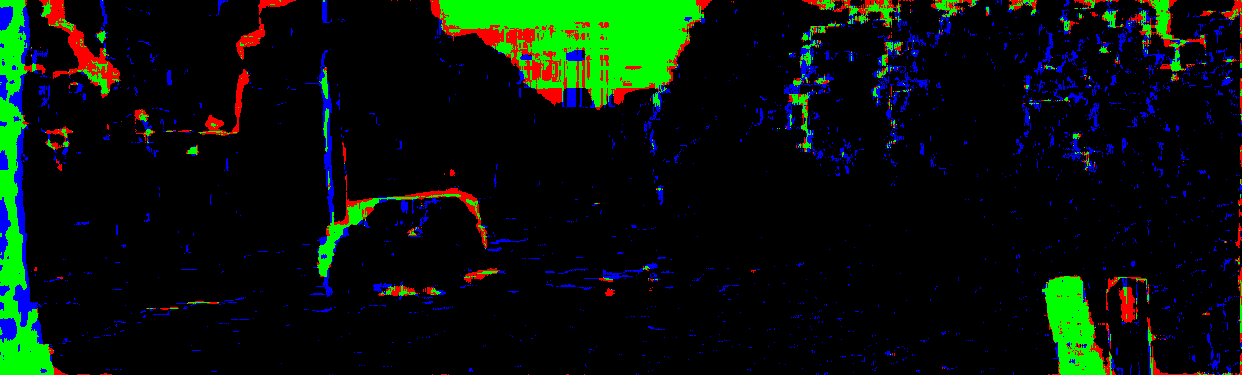
\includegraphics[width=0.99\linewidth]{Figures/Occ_56}
%                \caption{}
%        \end{subfigure}  
%        \caption{(a) \& (c) left image 003 \& 056 of KITTI 2015 training set, (b) \& (d) show pixels detected as ambiguous (threshold at $15$) with respect to LRC reference: true positive in green, over detection in red, and under-detection in blue.}
%\label{fig:occ} 
%\end{figure}

\begin{figure}
\centering        
        \begin{subfigure}[t]{0.98\linewidth}
                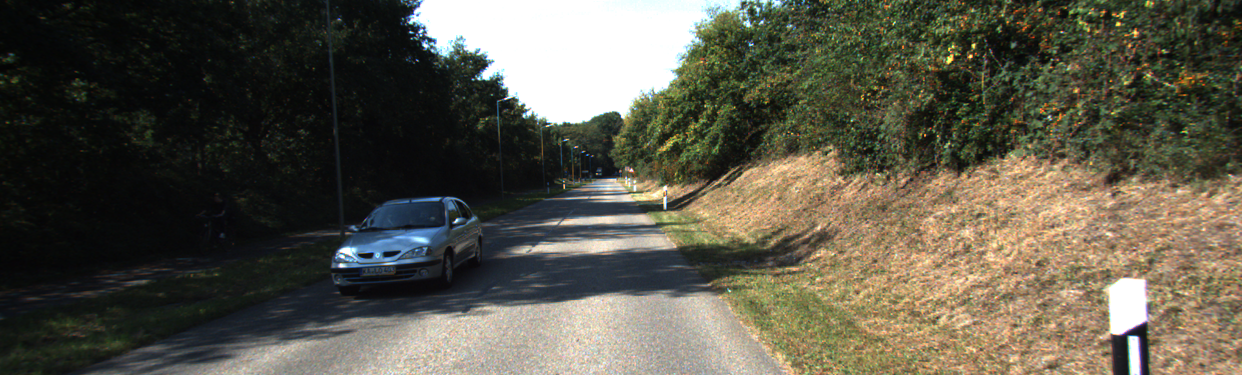
\includegraphics[width=0.99\linewidth]{Figures/56}
                \caption{}
        \end{subfigure}
        \begin{subfigure}[t]{0.98\linewidth}
                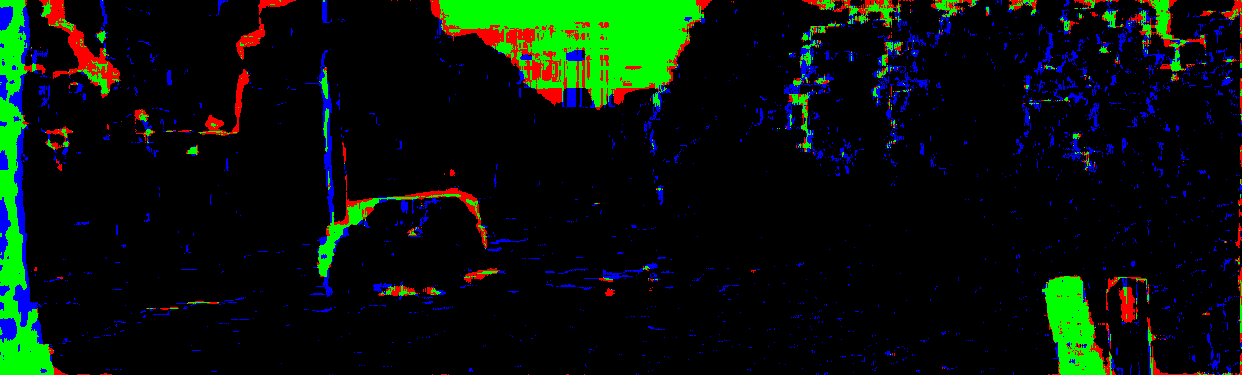
\includegraphics[width=0.99\linewidth]{Figures/Occ_56}
                \caption{}
        \end{subfigure}  
        \caption{(a) left image 056 of KITTI 2015 training set, (b) shows pixels detected as ambiguous (threshold at $15$) with respect to LRC reference: true positive in green, over detection in red, and under-detection in blue.}
\label{fig:occ} 
\end{figure}

On two scenes, Fig.\ref{fig:occ} shows pixels detected as with a high ambiguity index with respect to LRC labels ( ''correct'' or non ''correct''): true positive in green, false positive is red, false negative is blue and true negative is black. Most of occlusions are detected. Under-detection concerns thin objects or little discontinuities, and over-detection are mostly due to the right image objects not seen in the left image.

\subsection{Ambiguity index as data uncertainty}

\begin{figure}
\centering
        \begin{subfigure}[t]{0.98\linewidth}
                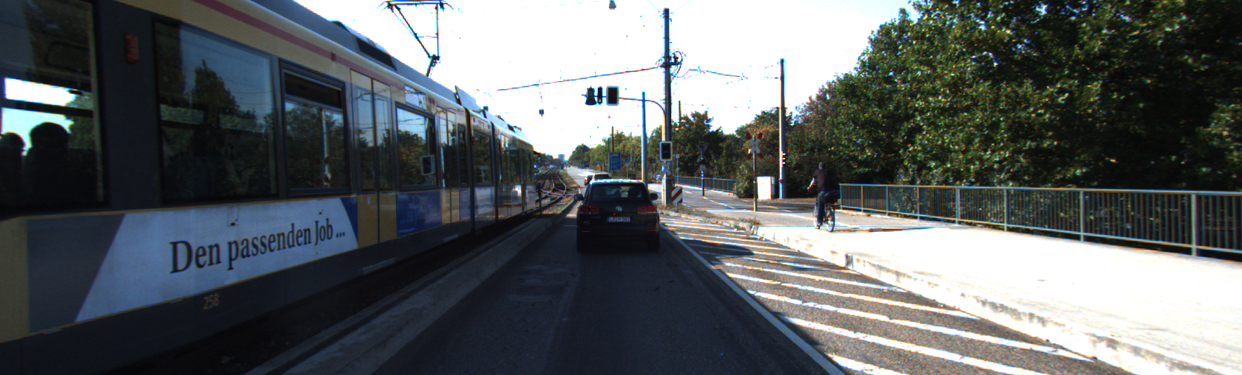
\includegraphics[width=0.99\linewidth]{Figures/144_10_il}
                \caption{Left image}
        \end{subfigure}
        \begin{subfigure}[t]{0.98\linewidth}
                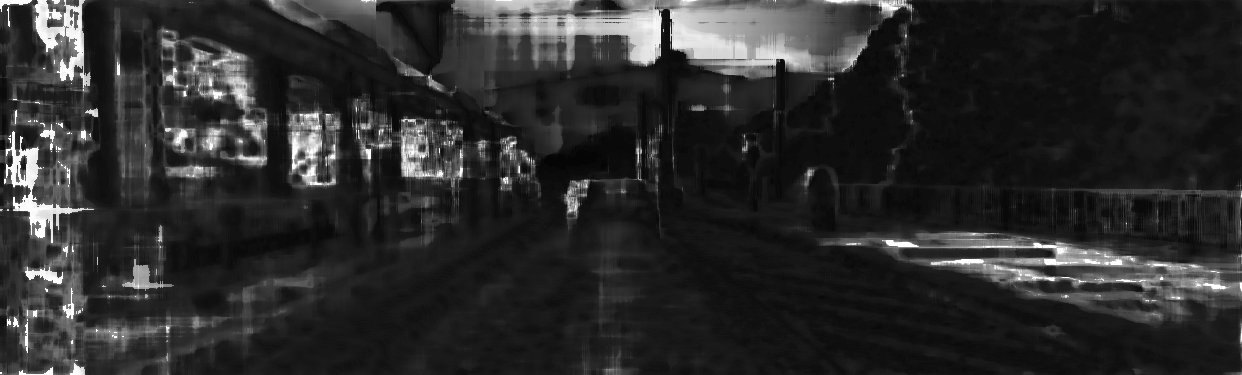
\includegraphics[width=0.99\linewidth]{Figures/144_10_ml2}
                \caption{Ambiguity index image}
        \end{subfigure}
        \begin{subfigure}[t]{0.98\linewidth}
                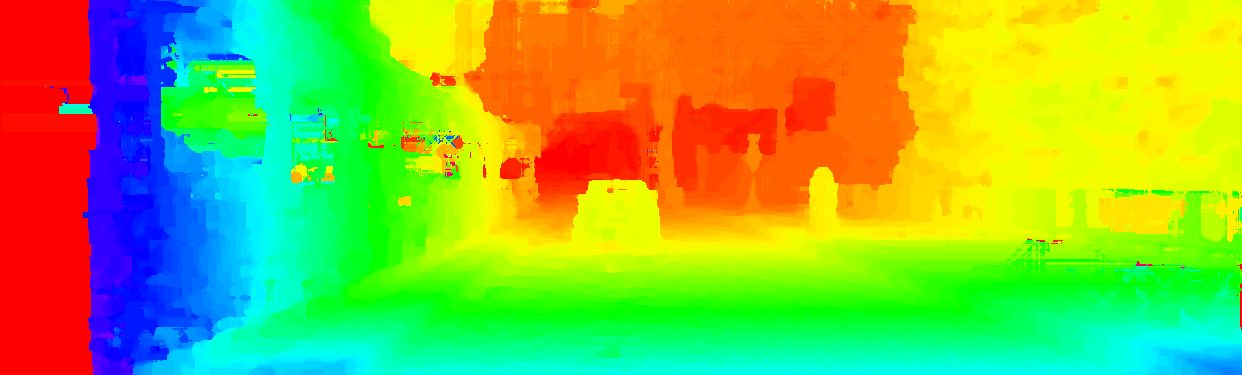
\includegraphics[width=0.99\linewidth]{Figures/144_10_df}
                \caption{Left disparity without index}
        \end{subfigure}        
        \begin{subfigure}[t]{0.98\linewidth}
                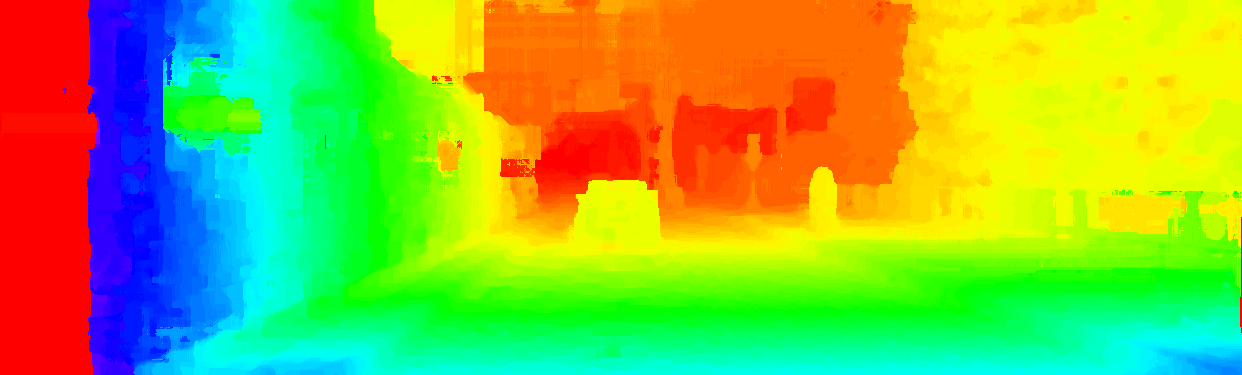
\includegraphics[width=0.99\linewidth]{Figures/144_10_df_}
                \caption{Left disparity with index weighting}
        \end{subfigure}        
        \caption{Results on image 144 of KITTI 2015 training set (a): Ambiguity index in (b), (c) disparity map without using the index, and (d) using the index. Higher is the index whiter is the index in (b).  Notice how reconstruction is improved on the tramway's glasses between (c) and (d).}
        \label{fig:disp}
\end{figure}

We tested the second refinement method proposed in sec.\ref{ss:in_proc} with $K=15$. Results are reported in the last line of Tab.~\ref{tab:KITTI}. What was obtained on the Refinement 1 method are confirmed with the Refinement 2 method, with the difference that combination of LRC and Refinement 2 leads to even better improvements. KITTI 2012, obtained error rate is ranked 37, and for KITTI 2015, it is ranked between 10 to 15 (in January 2017) witch is encouraging knowing that better data cost can be used.

A reconstruction result with and without the use of the index is shown Fig.\ref{fig:disp}, for illustration. Notice how the disparity map is improved on the tramway's glasses. The ambiguity index detects reflexions at the tramway's glasses, saturated pixels as in the sky and occlusion at the left of the car. Comparing result with and without weighting.

\section{Conclusion}
\label{sec:conclusion}

Our goal was to characterize the uncertainty of the disparity map which is estimated during stereo reconstruction process, which is known to be a necessary but difficult task to performed. We proposed an ambiguity index which is designed to approximate the variances of every pixels of the estimated disparity map. This ambiguity index can only be computed when Dynamic Programming is used to solve the stereo reconstruction problem, as it is the case for the well known SGM optimization. In the experiments, it was shown that the proposed index has higher values where the data does not match with the model, for example in case of occlusion and in presence of specularities. This allows to used the ambiguity index to improve the results by a post-processing, as shown experimentally with two proposed refinement methods on the KITTI 2012 and KITTI 2015 databases.  The proposed index can be also used for other kind of problems, until the optimization is based on Dynamic Programming.

% References should be produced using the bibtex program from suitable
% BiBTeX files (here: strings, refs, manuals). The IEEEbib.bst bibliography
% style file from IEEE produces unsorted bibliography list.
% -------------------------------------------------------------------------
\bibliographystyle{IEEEbib}
\bibliography{refs}

\end{document}
